\documentclass[11pt]{beamer}

\usepackage{cedilleverbatim}
\usepackage{times}
\usepackage[absolute,overlay]{textpos}
\usepackage{stmaryrd}
\usepackage{MnSymbol}
\usepackage[normalem]{ulem} %for \sout

\usepackage{tikz}
\usepackage{graphicx}
\usepackage{tabu}
%\usepackage{epstopdf}
\usepackage{color}
%\usepackage{tabularx}
\usepackage{pgflibraryarrows}
\usepackage{pgflibraryshapes}
\usepackage{pgfbaseimage}
\usepackage{listings}

\usetikzlibrary{decorations.text}

%\documentclass{beamer}
%\usepackage{beamerthemesplit}
%\usepackage{mathptmx}
%\usepackage{helvet}

%\usepackage{amsmath}
\usepackage{latexsym}
%\usepackage{amssymb}
\usepackage{proof}
\usepackage{verbatim} 
\usepackage{url}

\definecolor{navy}{RGB}{0,0,128}
\definecolor{dorange}{RGB}{255,100,0}
\definecolor{dgreen}{RGB}{0,75,0}
\definecolor{dbrown}{RGB}{125,30,0}
\definecolor{lbrown}{RGB}{245,150,120}
\definecolor{ored}{RGB}{255,150,70}
\definecolor{oredd}{RGB}{255,69,0}
\definecolor{lightred}{RGB}{255,70,70}
\definecolor{vlred}{RGB}{255,170,170}
\definecolor{cream}{RGB}{255,253,208}
\definecolor{lthistle}{RGB}{185,175,185}

\newcommand{\semeq}[1]{\langle\hspace{-.08cm}|#1|\hspace{-0.08cm}\rangle}
\newcommand{\rep}[1]{\ulcorner #1 \urcorner}
\newcommand{\tlift}[2]{{\uparrow}_{#1}\,(#2)}
\newcommand{\dstar}[0]{\smallstar}
\newcommand{\utp}[0]{\mathcal{U}}
\newcommand{\elcap}[0]{\cap}
\newcommand{\nutt}[4]{\nu\, #1\! :\! #2 \, |\, #3.\, #4}
\newcommand{\interp}[1]{\llbracket #1 \rrbracket} 
\newcommand{\abs}[4]{{#1}\, #2\! : \! #3.\, #4}

% unicode
\usepackage[utf8]{inputenc}
\DeclareUnicodeCharacter{2605}{\ensuremath{\star}}
\DeclareUnicodeCharacter{2081}{\ensuremath{_1}}
\DeclareUnicodeCharacter{2082}{\ensuremath{_2}}
\DeclareUnicodeCharacter{2228}{\ensuremath{\vee}}
\DeclareUnicodeCharacter{27E6}{\ensuremath{\llbracket}}
\DeclareUnicodeCharacter{27E7}{\ensuremath{\rrbracket}}
\DeclareUnicodeCharacter{228E}{\ensuremath{\uplus}}
\DeclareUnicodeCharacter{2113}{\ensuremath{\ell}}
\DeclareUnicodeCharacter{2294}{\ensuremath{\sqcup}}
\DeclareUnicodeCharacter{2192}{\ensuremath{\to}}
\DeclareUnicodeCharacter{2200}{\ensuremath{\forall}}
\DeclareUnicodeCharacter{22CE}{\ensuremath{\curlyvee}}
\DeclareUnicodeCharacter{2115}{\ensuremath{\mathbb{N}}}
\DeclareUnicodeCharacter{2238}{\ensuremath{\dotdiv}}
\DeclareUnicodeCharacter{2261}{\ensuremath{\equiv}}
\DeclareUnicodeCharacter{3BB}{\ensuremath{\lambda}}
\DeclareUnicodeCharacter{1D539}{\ensuremath{\mathbb{B}}}
\DeclareUnicodeCharacter{1D543}{\ensuremath{\mathbb{L}}}
\DeclareUnicodeCharacter{1D54A}{\ensuremath{\mathbb{S}}}
\DeclareUnicodeCharacter{1D54B}{\ensuremath{\mathbb{T}}}
\DeclareUnicodeCharacter{1D54D}{\ensuremath{\mathbb{V}}}
\DeclareUnicodeCharacter{D7}{\ensuremath{\times}}
\DeclareUnicodeCharacter{25C2}{\ensuremath{:}}

\newcommand{\myb}[0]{\ensuremath{\textcolor{blue}{\triangleright}}}

\newcommand{\fore}[0]{\ensuremath{F_\omega^{\textit{rec}}}}

\mathchardef\mhyph="2D % Define a "math hyphen"

\mode<presentation>
{
  %\usetheme{Warsaw}
  % or ...

%\usetheme{IowaCity}
\usetheme{Boston}
%\usetheme{Savannah}

%  \setbeamercovered{transparent}
  % or whatever (possibly just delete it)
}

\usepackage[english]{babel}
% or whatever

\usepackage{times}
\usepackage[T1]{fontenc}
% Or whatever. Note that the encoding and the font should match. If T1
% does not look nice, try deleting the line with the fontenc.



\date{\ }

\begin{document}


\setbeamercolor{normal text}{bg=white,fg=black}

\begin{frame}

\begin{center}
{\huge
  Introduction to Programming and

\vspace{.1cm}

  Proving in Cedille }

\vspace{.75cm}


\includegraphics[width=3cm]{logo}

%\includegraphics[width=5cm]{oldcap}

\vspace{.6cm}

Chris Jenkins, Colin McDonald, Aaron Stump

{\small
Computer Science 

The University of Iowa

Iowa City, Iowa
}

\end{center}
\end{frame}

\newcommand{\grun}[1]{\textcolor{dgreen}{\underline{#1}}}

\newcommand{\qlogo}[1]{\raisebox{-.25\height}{
\includegraphics[width=#1]{logo}}?}

\newenvironment{planslide}[2]{%
\begin{frame}
\frametitle{#2}

\large 

\begin{tabular}{l c l }

\qlogo{.7cm} &\ & \textcolor{#1}{Motivation and background for Cedille} \\ \\


$\vdash \textit{\textcolor{red}{C}e\textcolor{red}{D}i\textcolor{red}{L}l\textcolor{red}{E}}$ &\ & \textcolor{#1}{Syntax and semantics}\\ \\

\texttt{cedille} &\ & \textcolor{#1}{Tooling: emacs frontend $\leftrightarrow$ backend} \\ \\

$\leadsto\ \texttt{cedille}_{\texttt{core}}$ & \ & \textcolor{#1}{Elaboration to Cedille Core} \\ \\

\texttt{c d ll} &\ & \textcolor{#1}{Spine-local type inference} \\ \\ 

%\begin{tikzpicture}[
%  decoration={
%    reverse path,
%    text effects along path,
%    text={cedille cedille cedille cedille cedille cedille cedille cedille cedille cedille cedille cedille cedille cedille
%      cedille cedille cedille cedille cedille cedille cedille cedille cedille.},
%    text effects/.cd,
%      text along path,
%      character count=\i, character total=\n,
%      characters={scale=1-\i/\n}
%    }
%]
%\draw [decorate] (0,0) 
%    \foreach \i [evaluate={\r=(\i/2400)^2;}] in {0,7,...,2380}{ -- (\i:\r)}; 
%\end{tikzpicture}

\raisebox{-.8\height}{
\includegraphics[width=2cm]{cedillespiral}} &\ & 

\textcolor{#1}{Future directions}


\end{tabular}

\end{frame}
}



\planslide{white}{Plan for the tutorial}
\planslide{red}{Plan for the tutorial}

\begin{frame}
\begin{center}
  \Huge
  \qlogo{1.8
    cm}

  \vspace{1cm}

{\Large
  \textcolor{red}{Motivation and background for Cedille}
}
  \end{center}

\end{frame}

\begin{frame}
\frametitle{A little history}

\pause
\begin{center}

\includegraphics[width=4in]{bonnevillesign}
\end{center}

\end{frame}

\setlength{\TPHorizModule}{.1cm}
\setlength{\TPVertModule}{.1cm}
\setbeamercolor{mycolor}{fg=black,bg=white}

\newcommand{\carbox}[4]{%
\begin{tikzpicture}
    \node at (0,0) {#1};
    \node at (-2.68,-4.2) {\small \emph{#4}};
    \pause
    \node at #2 {#3};

\end{tikzpicture}
}

\begin{frame}
  \frametitle{System F (Girard, Reynolds, early 1970s)}

  \carbox{
\includegraphics[width=4in]{bonneville1}}{(0,2.5)}{\begin{minipage}{7cm}
  \begin{beamercolorbox}{mycolor}
        \begin{itemize}
        \item[$\myb$] $\forall\ X : \star.\ T$
        \item[$\myb$] Raw power (\textcolor{blue}{impredicativity!})
        \item[$\myb$] A little crude (\textcolor{red}{no Curry-Howard})
          \vspace{.25cm}
          \end{itemize}
                    \end{beamercolorbox}\end{minipage}}{1969 Mercury Cyclone Spoiler II}

    \end{frame}

\begin{frame}
  \frametitle{Calculus of Constructions (Coquand, Huet 1988)}

  \carbox{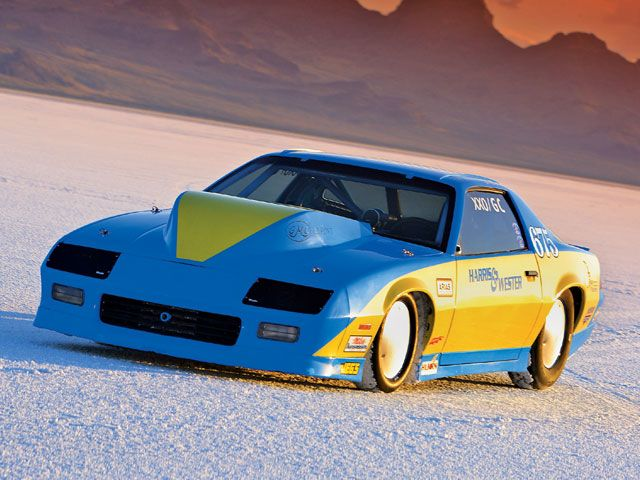
\includegraphics[width=4in]{camaro}}{(0,2.4)}{\begin{minipage}{9cm}
      \begin{beamercolorbox}{mycolor}
        \begin{itemize}
        \item[$\myb$] Add dependent types: $\Pi\ x : T.\ T'$
        \item[$\myb$] Imported from Automath/Martin-L\"of type theory
        \item[$\myb$] \textcolor{blue}{Curry-Howard!}
        \item[$\myb$] \textcolor{red}{No induction.} [Geuvers 2001]
        \end{itemize}
        \end{beamercolorbox}\end{minipage}}{1988 Chevrolet Camaro}

\end{frame}

\begin{frame}
  \frametitle{Calculus of Inductive Constructions (Werner 1994)}

  \carbox{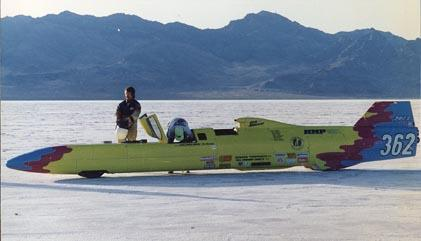
\includegraphics[width=4in]{streamliner}}{(0,1.8)}{\begin{minipage}{9cm}
      \begin{beamercolorbox}{mycolor}
        \begin{itemize}
        \item[$\myb$] Add primitive inductive types
        \item[$\myb$] Finally ready for constructive mathematics!
        \item[$\myb$] Basis for Coq
        \end{itemize}
        \end{beamercolorbox}\end{minipage}}{1992 Hoffman-Markley Streamliner}
\end{frame}

\begin{frame}
  \frametitle{But Coq $\neq$ CIC}

  \begin{itemize}
  \item[$\myb$] Coinductive types
  \item[$\myb$] Universe hierarchy (Extended CC, Luo 1990)
  \item[$\myb$] Proof-irrelevant universe \texttt{Prop}
  \item[$\myb$] \emph{And we might want more:}
    \begin{itemize}
    \item definitional proof irrelevance
    \item inductive-inductive types
    \item inductive-recursive types
      \end{itemize}
  \end{itemize}

\vspace{.5cm}

  Similarly, Agda $\neq$ MLTT.

\vspace{.5cm}

\end{frame}

\begin{frame}
  \frametitle{Issues and limitations, Coq and Agda}

  \begin{itemize}
  \item[$\myb$] No formal semantics/correctness proof
    \begin{itemize}
    \item Despite a lot of interest: TT in TT
      \end{itemize}

\vspace{.1cm}

  \item[$\myb$] (\textcolor{blue}{Hence!}) bugs and surprises
    \begin{itemize}
    \item[$\myb$] incompatibilities with various axioms
    \item[$\myb$] actual contradictions!
    \item[$\myb$] type soundness broken in Coq
    \end{itemize}

\vspace{.1cm}

  \item[$\myb$] Commitment to a set of datatypes
    \begin{itemize}
      \item[$\myb$] theory of datatypes not finished...
      \item[$\myb$] e.g., higher-order abstract syntax prohibited
    \end{itemize}
  \end{itemize}
\end{frame}

\newcommand{\monsterf}[1]{\begin{frame}
  \frametitle{Have we created a monster?}

  \includegraphics[width=4.5in]{#1}

  {\small \emph{Schaufelradbagger 258}}

\end{frame}
}

\monsterf{bagger258a}
\monsterf{bagger258b}

\begin{frame}
  \frametitle{\emph{If I could turn back time...}}

  \begin{columns}
\hspace{.5cm}    \column{2.8in}

  Good-bye to:

  \begin{itemize}
  \item[$\myb$] primitive datatypes
  \item[$\myb$] (also universe hierarchy, my bias)
  \end{itemize}

\vspace{.2cm}

  Hello to

  \begin{itemize}
  \item[$\myb$] lambda-encodings of data
  \end{itemize}

  \column{2.6in}
  \onslide<2>{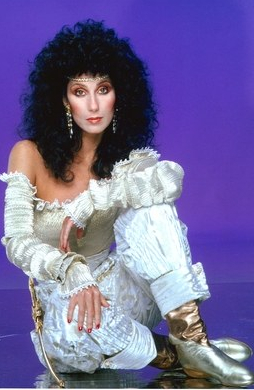
\includegraphics[width=1.8in]{cher}}
  \end{columns}

  \onslide<3>{\ }
  \end{frame}

\begin{frame}
  \frametitle{\colorbox{black}{\textcolor{white}{Wanted}}: \textcolor{red}{a new type theory} }

  where

  \begin{itemize}
  \item[$\myb$] inductive datatypes are \underline{derived} (lambda-encoded)
  \item[$\myb$] impredicativity is central
  \item[$\myb$] core theory is small and verifiable
  \end{itemize}

\vspace{.15cm}

  Tooling goals:

  \begin{itemize}
  \item[$\myb$] see all typing/inference information 
  \item[$\myb$] predictable inference
  \item[$\myb$] elaborate to core with independent checker
  \end{itemize}

\end{frame}

\begin{frame}
  \frametitle{Introducing Cedille}
\begin{center}

  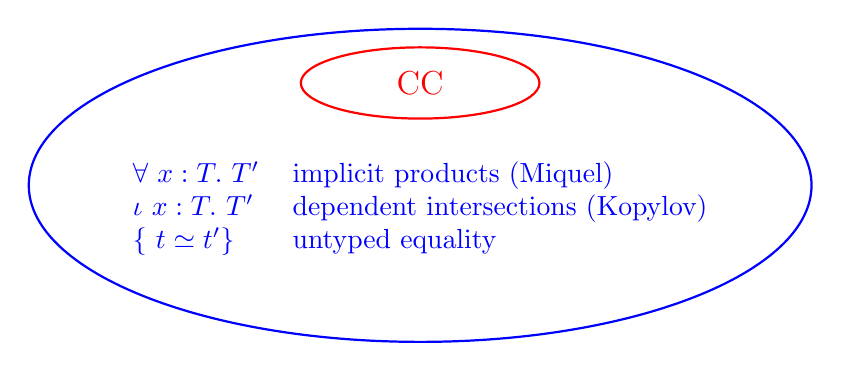
\begin{tikzpicture}
    \path (0,.3) node[ellipse,inner xsep=22pt,draw,inner ysep=5pt,red,thick](cc){\large CC} ;
    \path (0,-1) node[ellipse,inner xsep=100pt,draw,inner ysep=40pt,blue,thick](extcirc){\ };
    \path (0,-1.3) node{\color{blue}
        \begin{tabular}{ll}
          $\forall\ x : T.\ T'$ & implicit products (Miquel) \\
          $\iota\ x : T .\ T'$ & dependent intersections (Kopylov) \\
          $\{\ t \simeq t' \}$ & untyped equality
          \end{tabular}};
    \end{tikzpicture}

  \begin{itemize}
  \item[$\myb$] Small theory, formal syntax and semantics
  \item[$\myb$] Core checker implemented in $<1000$loc Haskell
  \item[$\myb$] Logically sound
  \item[$\myb$] Turing complete(!)
  \item[$\myb$] Supports inductive lambda-encodings
    \end{itemize}

\end{center}

  \end{frame}

\begin{frame}
  \frametitle{Back the truck up}
  \pause
\vspace{2cm}
\begin{tikzpicture}
    \node at (0,0) {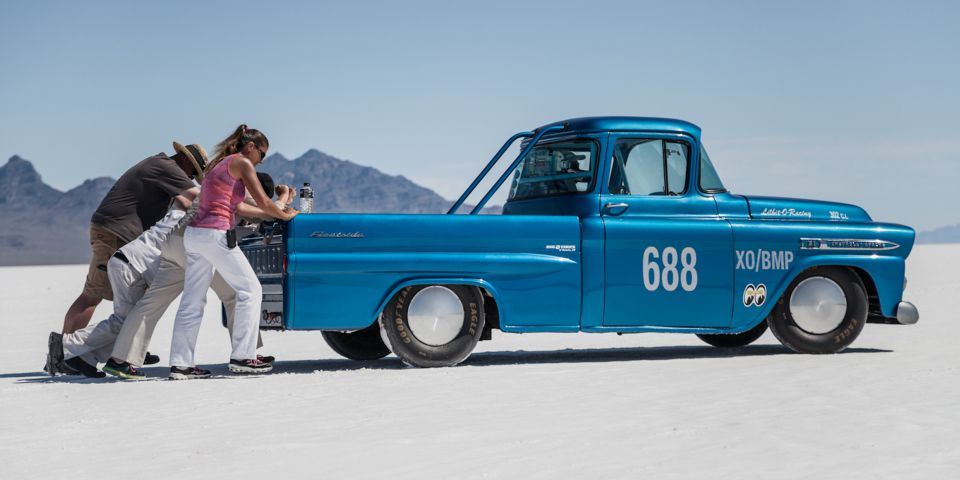
\includegraphics[width=4.3in]{bonnevillestuck}};
    \node at (0,2) {\begin{minipage}{8cm}\Large \color{white}Did you say lambda encodings?\end{minipage}};
\end{tikzpicture}

\end{frame}

\begin{frame}
  \frametitle{Not your forebear's lambda encodings}

  \begin{itemize}
  \item[$\myb$] Usual rap: inefficient accessors
  \item[$\myb$] Corrected by Parigot 1988 for typed encoding
  \item[$\myb$] \underline{Perfect} untyped encoding B\"ohm et al. 1994
    \begin{itemize}
    \item linear space
    \item constant-time accessors
    \item intrinsic support for iteration
    \end{itemize}
  \item[$\myb$] Cedille: perfect inductive (typed) encodings
  \end{itemize}

  \end{frame}

\begin{frame}
  \frametitle{What do we get from this?}
  
\begin{tikzpicture}
    \node at (0,0) {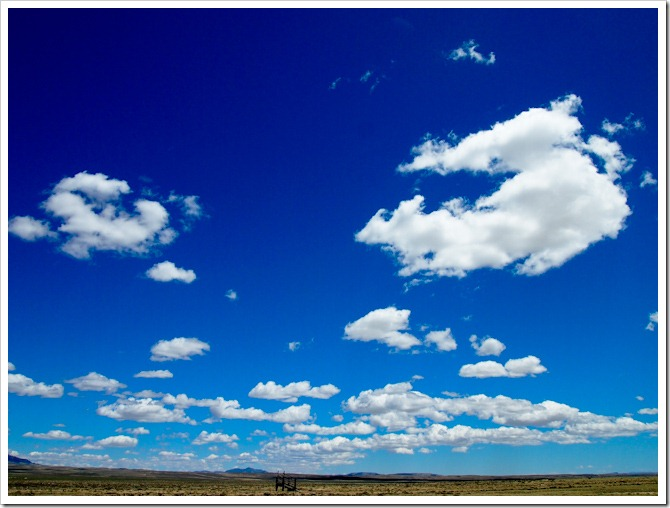
\includegraphics[width=4.3in]{Big-sky-Wyoming}};
\pause
\node at (0,2) {\begin{minipage}{8cm}
\vspace{1cm}
    
\Large \color{white}\emph{Freedom}

\pause

\vspace{1cm}

    \begin{beamercolorbox}{mycolor}
\normalsize
      \begin{itemize}
      \item[$\myb$] No pre-set datatype class
      \item[$\myb$] Explore semantics of advanced datatypes
      \item[$\myb$] \emph{Power of impredicativity}
      \item[$\myb$] So far: Functorial, Monotone, IR, II
      \end{itemize}
      \end{beamercolorbox}
\end{minipage}};
\end{tikzpicture}
\end{frame}

\begin{frame}
  \frametitle{So which car are we?}

  \pause

\begin{tikzpicture}
    \node at (0,0) {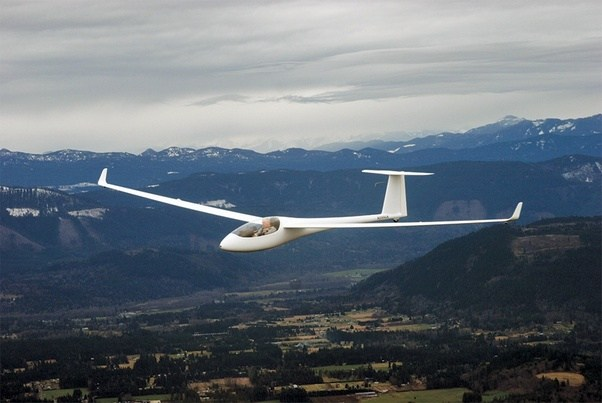
\includegraphics[width=4.3in]{glider}};
\pause
\node at (0,3) {\begin{minipage}{8cm}
\vspace{1cm}
    
\large \color{white}Elegant, at present a little in the clouds
\end{minipage}};
\end{tikzpicture}

  \end{frame}

\begin{frame}
\begin{center}
{
  \Huge
  $\vdash \textit{\textcolor{red}{C}e\textcolor{red}{D}i\textcolor{red}{L}l\textcolor{red}{E}}$
}

\vspace{1cm}

\Large

\textcolor{black}{Syntax and semantics of Cedille}

\vspace{.5cm}

{\small
\textcolor{red}{Calculus of Dependent Lambda Eliminations}}
\end{center}
\end{frame}


%\tabulinesep=1.2mm

\begin{frame}
\frametitle{CDLE}
\begin{center}
  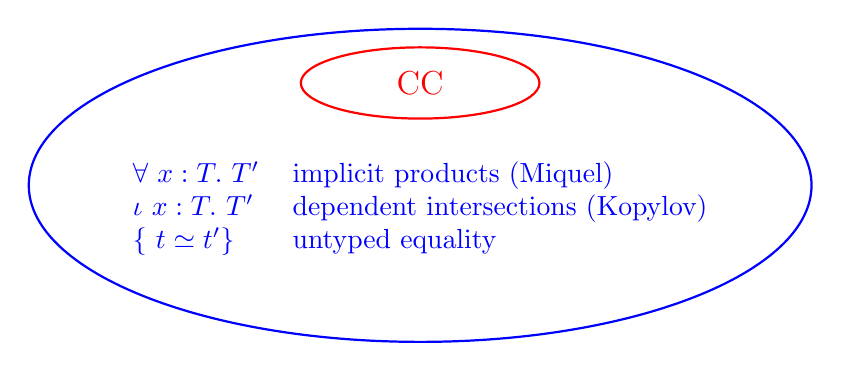
\begin{tikzpicture}
    \path (0,.3) node[ellipse,inner xsep=22pt,draw,inner ysep=5pt,red,thick](cc){\large CC} ;
    \path (0,-1) node[ellipse,inner xsep=100pt,draw,inner ysep=40pt,blue,thick](extcirc){\ };
    \path (0,-1.3) node{\color{blue}
        \begin{tabular}{ll}
          $\forall\ x : T.\ T'$ & implicit products (Miquel) \\
          $\iota\ x : T .\ T'$ & dependent intersections (Kopylov) \\
          $\{\ t \simeq t' \}$ & untyped equality
          \end{tabular}};
  \end{tikzpicture}
  \end{center}
\end{frame}

\begin{frame}
  \frametitle{Dependent intersections $\iota\ x:T_1.\ T_2$}

  \begin{itemize}
  \item[$\myb$] Usual intersection types:

    \[
    \infer{t : T_1 \cap T_2}{t : T_1 \qquad t : T_2}
    \]

    \item[$\myb$] Dependent intersection:

    \[
    \infer{t : \iota\ x : T_1 .\ T_2}{t : T_1 \qquad t : [t/x]T_2}
    \]

  \end{itemize}
  
\vspace{.3cm}

  \begin{center}
    \color{purple}
    \fbox{$T_2$ can refer to subject of typing, at weaker type $T_1$}
  \end{center}
  \end{frame}

\begin{frame}
  \frametitle{But if you are using intersections...\raisebox{-.15\height}{
\includegraphics[width=.7cm]{lightbulb}}}

  \pause

  You must have an \textcolor{red}{extrinsic} (Curry-style) type theory.

  \vspace{.25cm}

  \begin{itemize}
\pause
  \item[$\myb$] Unannotated terms of pure lambda calculus
\pause
  \item[$\myb$] Assign multiple different types to same term

 (Intrinsic type theories usually have unique types.)

\pause
  \item[$\myb$] Completely different from Coq, Agda
\pause
  \item[$\myb$] Much less explored TT...
  \end{itemize}
  

  \pause

\vspace{1cm}

  {\Large \color{red} Yes!}
\end{frame}
  
\begin{frame}
  \frametitle{For each type (here, implicit products)}

  \begin{itemize}
  \item[$\myb$] Formation rule for the type
{\small
    \[
    \infer{\Gamma\vdash \forall\ x : T'.\ T : \star}{\Gamma\vdash T':\star \qquad \Gamma,x:T'\vdash T : \star}
    \]
}

\vspace{-.5cm}

  \item[$\myb$] Introduction and elimination rules
{\small
    \[
    \begin{array}{ll}
      \infer{\Gamma \vdash t : \forall\ x : T'.\ T}{\Gamma \vdash \forall\ x : T' .\ T : \star \qquad \Gamma, {\color{red}x : T'} \vdash t : T} &
    \infer{\Gamma\vdash t : [t'/x]T}{\Gamma \vdash t : \forall\ x : T'.\ T \qquad \Gamma \vdash {\color{blue}t' : T'}}      
    \end{array}
    \]
}
     
\vspace{-.25cm}

  \item[$\myb$] Annotated terms

    \begin{itemize}
    \item Introduction: ${\color{red}\Lambda\ x : T'.}\ t$
    \item Elimination: $t\ {\color{blue}-t'}$
    \end{itemize}

\vspace{.2cm}

  \item[$\myb$] Annotated terms erase to pure lambda terms
    \begin{eqnarray*}
      |\Lambda\ x : T.\ t| & = & |t| \\
      |t\ \mhyph t'| & = & |t|
    \end{eqnarray*}
  \end{itemize}

\vspace{-4.3cm}


\hspace{4cm}  
\begin{tikzpicture}
  \draw[->,very thick,red] (2,-.7) -- (2.6,.65);
  \end{tikzpicture}

\vspace{4.5cm}


\end{frame}

\begin{frame}
  \frametitle{Equality type}

  \underline{Formation:}

  \[
  \infer{\Gamma \vdash \{ t \simeq t' \} : \star}{\textit{FV}(t\ t')\subseteq\textit{dom}(\Gamma)}
  \]

  \underline{Introduction and elimination:}
  \[
  \begin{array}{ll}
    \infer{\Gamma\vdash \textcolor{purple}{t} : \{ t' \simeq t'\}}{\textit{FV}(t')\subseteq\textit{dom}(\Gamma)}
    &
    \infer{\Gamma\vdash t : [t_2/x]T}{\Gamma\vdash t' : \{ t_1\simeq t_2\} \qquad \Gamma\vdash t : [t_1/x]T}
  \end{array}
  \]

\vspace{.1cm}

  \underline{Direct computation rule:}
  \[
  \infer{\Gamma\vdash t_2 : T}{\Gamma\vdash t : \{ t_1 \simeq t_2\} \qquad \Gamma\vdash t_1 : T}
  \]

  \underline{Annotations:}
  \begin{eqnarray*}
    |\beta\{\textcolor{purple}{t}\}| & = & |t| \\
    |\rho\ t'\ \mhyph\ t| & = & |t| \\
    |\phi\ t\ \mhyph\ t_1\{t_2\}| & = & |t_2|
  \end{eqnarray*}


\vspace{-4.5cm}


\hspace{2.2cm}  \begin{tikzpicture}
  \draw[->,very thick,purple] (2.85,-2) -- (-0.6,.7);
  \end{tikzpicture}

\vspace{4.5cm}
\end{frame}  

\begin{frame}
  \frametitle{The Kleene trick}

  \begin{itemize}
  \item[$\myb$] Any term can be assigned a trivially true equality
\[
    \colorbox{purple}{\textcolor{white}{t}} : \{ t' \simeq t'\}
\]

  \item[$\myb$] Restricted form of subset type,  combined with \emph{conversion}

    \[
    \infer{\Gamma\vdash t : T}{\Gamma \vdash t:T' \qquad \Gamma \vdash T : \star \qquad T \cong T'}
    \]

  \item[$\myb$] When $[t/x]t' =_{\beta\eta} [t/x]t''$, yields

    \[
    t : {\color{red}\iota\ x : T.\ \{ t' \simeq t'' \}}
    \]

  \item[$\myb$] E.g.,
    \begin{eqnarray*}
      \textit{True} & = & \forall\ X : \star.\ X \to X \\
      \lambda\ y.\ y\ y & : & {\color{red}\iota\ x : \textit{True} \to \textit{True}.\ \{ x\ \lambda\, z.z \simeq \lambda\, z.z \}} \\ 
      \textit{anything} & : & \{ \lambda\, x.x \simeq \lambda\, x.x \}
    \end{eqnarray*}
    

  \end{itemize}
\end{frame}

\begin{frame}
  \frametitle{Aside on rewriting}

  \begin{center}
    \huge
    \colorbox{purple}{$\color{white}\rho\ t\ \mhyph\ t'$}
  \end{center}

  \begin{itemize}
    \item[$\myb$]  Suppose $t : \{ t_1 \simeq t_2 \}$, and $T$ is type for $t'$.

    \item[$\myb$]  Find each subterm of $T$ convertible to $t_1$ and rewrite.
    \item[$\myb$] Error if no matches
    \item[$\myb$] Use $\rho$ anywhere in a term (cf. Agda)
    \item[$\myb$] Other forms of $\rho$:
      \begin{itemize}
      \item $\rho+$, head-normalize as you look for matches
      \item $\rho\langle n_1 \cdots n_k \rangle$, rewrite occurrences $n_1,\cdots n_k$
      \end{itemize}
  \end{itemize}
\end{frame}

  
    

\begin{frame}
  \frametitle{Dependent intersections}

  \underline{Formation:}
  \[
  \infer{\Gamma\vdash \iota\ x:T.\ T'}{\Gamma\vdash T:\star \qquad \Gamma,x:T\vdash T':\star}
  \]

  \underline{Introduction and elimination:}
  \[
  \begin{array}{ll}
  \infer{\Gamma\vdash t : \iota\ x:T.\ T'}{\Gamma\vdash t : T \qquad \Gamma\vdash \textcolor{blue}{t} : [t/x]T'}
  &
  \infer{\Gamma\vdash t : T}{\Gamma\vdash t : \iota\ x:T.\ T'} \ \
  \infer{\Gamma\vdash t : [t/x]T'}{\Gamma\vdash t : \iota\ x:T.\ T'}
  \end{array}
  \]

  \underline{Annotations:}
  \begin{eqnarray*}
    |[t,\textcolor{blue}{t'}]| & = & |t| \\
    |t.1| & = & |t| \\
    |t.2| & = & |t|
  \end{eqnarray*}
\end{frame}

\begin{frame}
  \frametitle{How are inductive datatypes defined?}

  \begin{itemize}
  \item[$\myb$] Several variations (CPP '18, ITP '18), one theme:

    \vspace{.2cm}
    
{\color{blue}
    The type of $d$ expresses an induction principle for $d$ 
}

    \vspace{.2cm}


  \item[$\myb$] For Nat:
    \[
    n\ :\ \forall\ P : \textit{Nat} \to \star.\ (\forall\ x:\textit{Nat}.\ P\ x \to P\ (S\ x)) \to P\ Z \to P\ n
    \]
    
  \item[$\myb$] Essentially due to Leivant 1983
  \item[$\myb$] Will walk through example a little later
  \item[$\myb$] With D. Firsov, generic derivations for classes of $F : \star \to \star$
  \end{itemize}
\end{frame}

\begin{frame}[containsverbatim]
  \frametitle{Another example: casts}

  \begin{itemize}
  \item[$\myb$] A cast is an identity function from A to B

{\small
\begin{verbatim}
Cast ◂ ★ ➔ ★ ➔ ★ = λ A : ★ . λ B : ★ .
   ι cast : A ➔ B . { cast ≃ λ x . x }.
\end{verbatim}
}

\item[$\myb$] If there is a cast, you can change the type:

{\small
\begin{verbatim}
cast ◂ ∀ A : ★ . ∀ B : ★ . Cast · A · B ➾ A ➔ B 
  = ...
\end{verbatim}
}

\item[$\myb$] Nontrivial casts exist in extrinsic type theory:

\vspace{-.2cm}

\[ {\color{red}\lambda\ x.\,x} \ \ : \ \ (\abs{\forall}{X}{\star}{X\to X}) \to (\textit{Nat} \to \textit{Nat}) \]

\item[$\myb$] Not in intrinsic type theory:

\vspace{-.2cm}

\[ {\color{red}\lambda\ x.\,(x \cdot \textit{Nat})} \ \ : \ \ (\abs{\forall}{X}{\star}{X\to X}) \to (\textit{Nat} \to \textit{Nat}) \]

  \end{itemize}

  \end{frame}

\begin{frame}
  \frametitle{Monotone recursive types}

  \begin{itemize}
  \item[$\myb$] Explored in works by R. Matthes \textcolor{purple}{[eg, in Synthese, 2002]}

\vspace{.1cm}

  \item[$\myb$] Given \underline{monotone} $F$, extend the theory with $\mu F$

\vspace{.1cm}

  \item[$\myb$] Monotonicity expressed by a term t of type

\vspace{.2cm}

    \hspace{.1cm} $ \abs{\forall}{X}{\star}{\abs{\forall}{Y}{\star}{(X \to Y) \to (F\cdot X \to F\cdot Y)}} $

\vspace{.1cm}

  \item[$\myb$] Matthes considers how to extend theory, retaining SN

    \pause

\vspace{1cm}

{\large
    \textcolor{blue}{\emph{We can derive a stronger form, within our theory!}}
}
  \end{itemize}
 \end{frame}
        
\begin{frame}
  \frametitle{Starting point: proof of Tarski's Theorem}

  Consider monotone $f : \mathcal{P}(X) \to \mathcal{P}(X)$

\vspace{1cm}

  Let $Q = \bigcap\{ A\ |\ f(A) \subseteq A\}$

\vspace{1cm}

  Prove $f(Q) = Q$ by both inclusions.

  \end{frame}
    
\begin{frame}[containsverbatim]
  \frametitle{Translating the proof to Cedille}

  \begin{itemize}
  \item[$\myb$] ``$A \subseteq B$'' becomes \verb|Cast · A · B|

    \vspace{.75cm}

  \item[$\myb$] Monotonicity becomes

    {\footnotesize
\begin{verbatim}
∀ X : ★ . ∀ Y : ★ . 
Cast · X · Y ➔ Cast · (F · X) · (F · Y) 
\end{verbatim}
}

    \vspace{.75cm}

  \item[$\myb$] ``$\bigcap\{ A\ |\ f(A) \subseteq A\}$'' becomes

{\footnotesize
\begin{verbatim}
Rec = ∀ X : ★ . Cast · (F · X) · X ➾ X 
\end{verbatim}
}

\end{itemize}
\end{frame}

\begin{frame}[containsverbatim]
  \frametitle{Monotone recursive types: summary}

  \begin{itemize}
  \item[$\myb$] Derive \verb|Rec| for any monotone \verb|F|
    \item[$\myb$] Casts (identity functions) between \verb|F · Rec| and \verb|Rec|
    \item[$\myb$] Proof translates proof of Tarski fixed-point theorem
    \item[$\myb$] Code is 18 lines of Cedille
\item[$\myb$] \underline{To emphasize:} no addition to the theory, these are derived
      \end{itemize}
\end{frame}

\begin{frame}
\begin{center}
{  \Huge
\texttt{cedille}}

  \vspace{1cm}

{\Large
  \textcolor{red}{Tooling: emacs frontend $\leftrightarrow$ backend}

  \vspace{3cm}

  \url{cedille.github.io}
}
  \end{center}

\end{frame}

\begin{frame}
\frametitle{Emacs mode}

\begin{itemize}
\item[$\myb$] Interact with Cedille through an emacs mode

\vspace{.25cm}

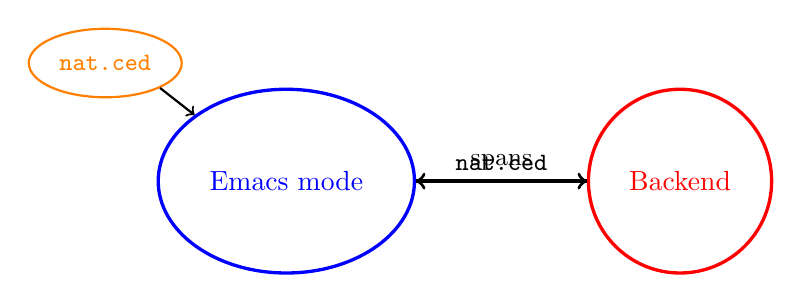
\begin{tikzpicture}

\path (1,2.5) node[very thick,blue,ellipse,draw,inner xsep=5pt,inner ysep=20pt](emacsmode){Emacs mode} ;
\path (6,2.5) node[very thick,red,ellipse,draw,inner xsep=5pt,inner ysep=20pt](backend){Backend} ;

\path (-1.3,4) node[thick,orange,ellipse,draw,inner xsep=3pt,inner ysep=6pt](cedfilesa){{\small \texttt{nat.ced}}} ;

\draw[->,thick,black] (cedfilesa.south east) -- (emacsmode.north west);
\onslide<1>{\draw[->,very thick,black] (emacsmode.east) -- node[pos=0.5,above]{\small \texttt{nat.ced}} (backend.west);}
\onslide<2>{\draw[<-,very thick,black] (emacsmode.east) -- node[pos=0.5,above]{\small spans} (backend.west);}

\end{tikzpicture}

\pause
\vspace{.1cm}

\item[$\myb$] A span is $[\textit{label},\textit{start-pos},\textit{end-pos},\textit{attributes}]$

\item[$\myb$] Spans communicated in JSON

\item[$\myb$] Cedille sends \underline{all} type information, in span attributes

\item[$\myb$] Monadic style for writing the backend (type checker)

\end{itemize}
\end{frame}

\begin{frame}
\begin{center}
\vspace{3cm}
{  \Huge
Demo \texttt{cedille}}

  \vspace{1cm}

  \end{center}

\end{frame}


\end{document}
